\chapter{场景模型}

    在实验部分(第\ref{sec:experiment}章)中, 为三个被测服务, 均设计了场景模型.
    
    虽然场景模型允许概率性的初始状态与终止状态分布, 但在这些场景模型中只用到了确定性的初始状态与终止状态. 未标数字的转移边表示概率权值在出边中均等分布.
    
    \section{OSS服务测试场景模型}
        OSS服务(云对象存储服务)的场景模型共有3个, 分别为Scenario A(图\ref{fig:oss_scenario_A}), Scenario B(图\ref{fig:oss_scenario_B})和Scenario C(图\ref{fig:oss_scenario_C}).
        
        \begin{figure}[!htb]
            \centering
            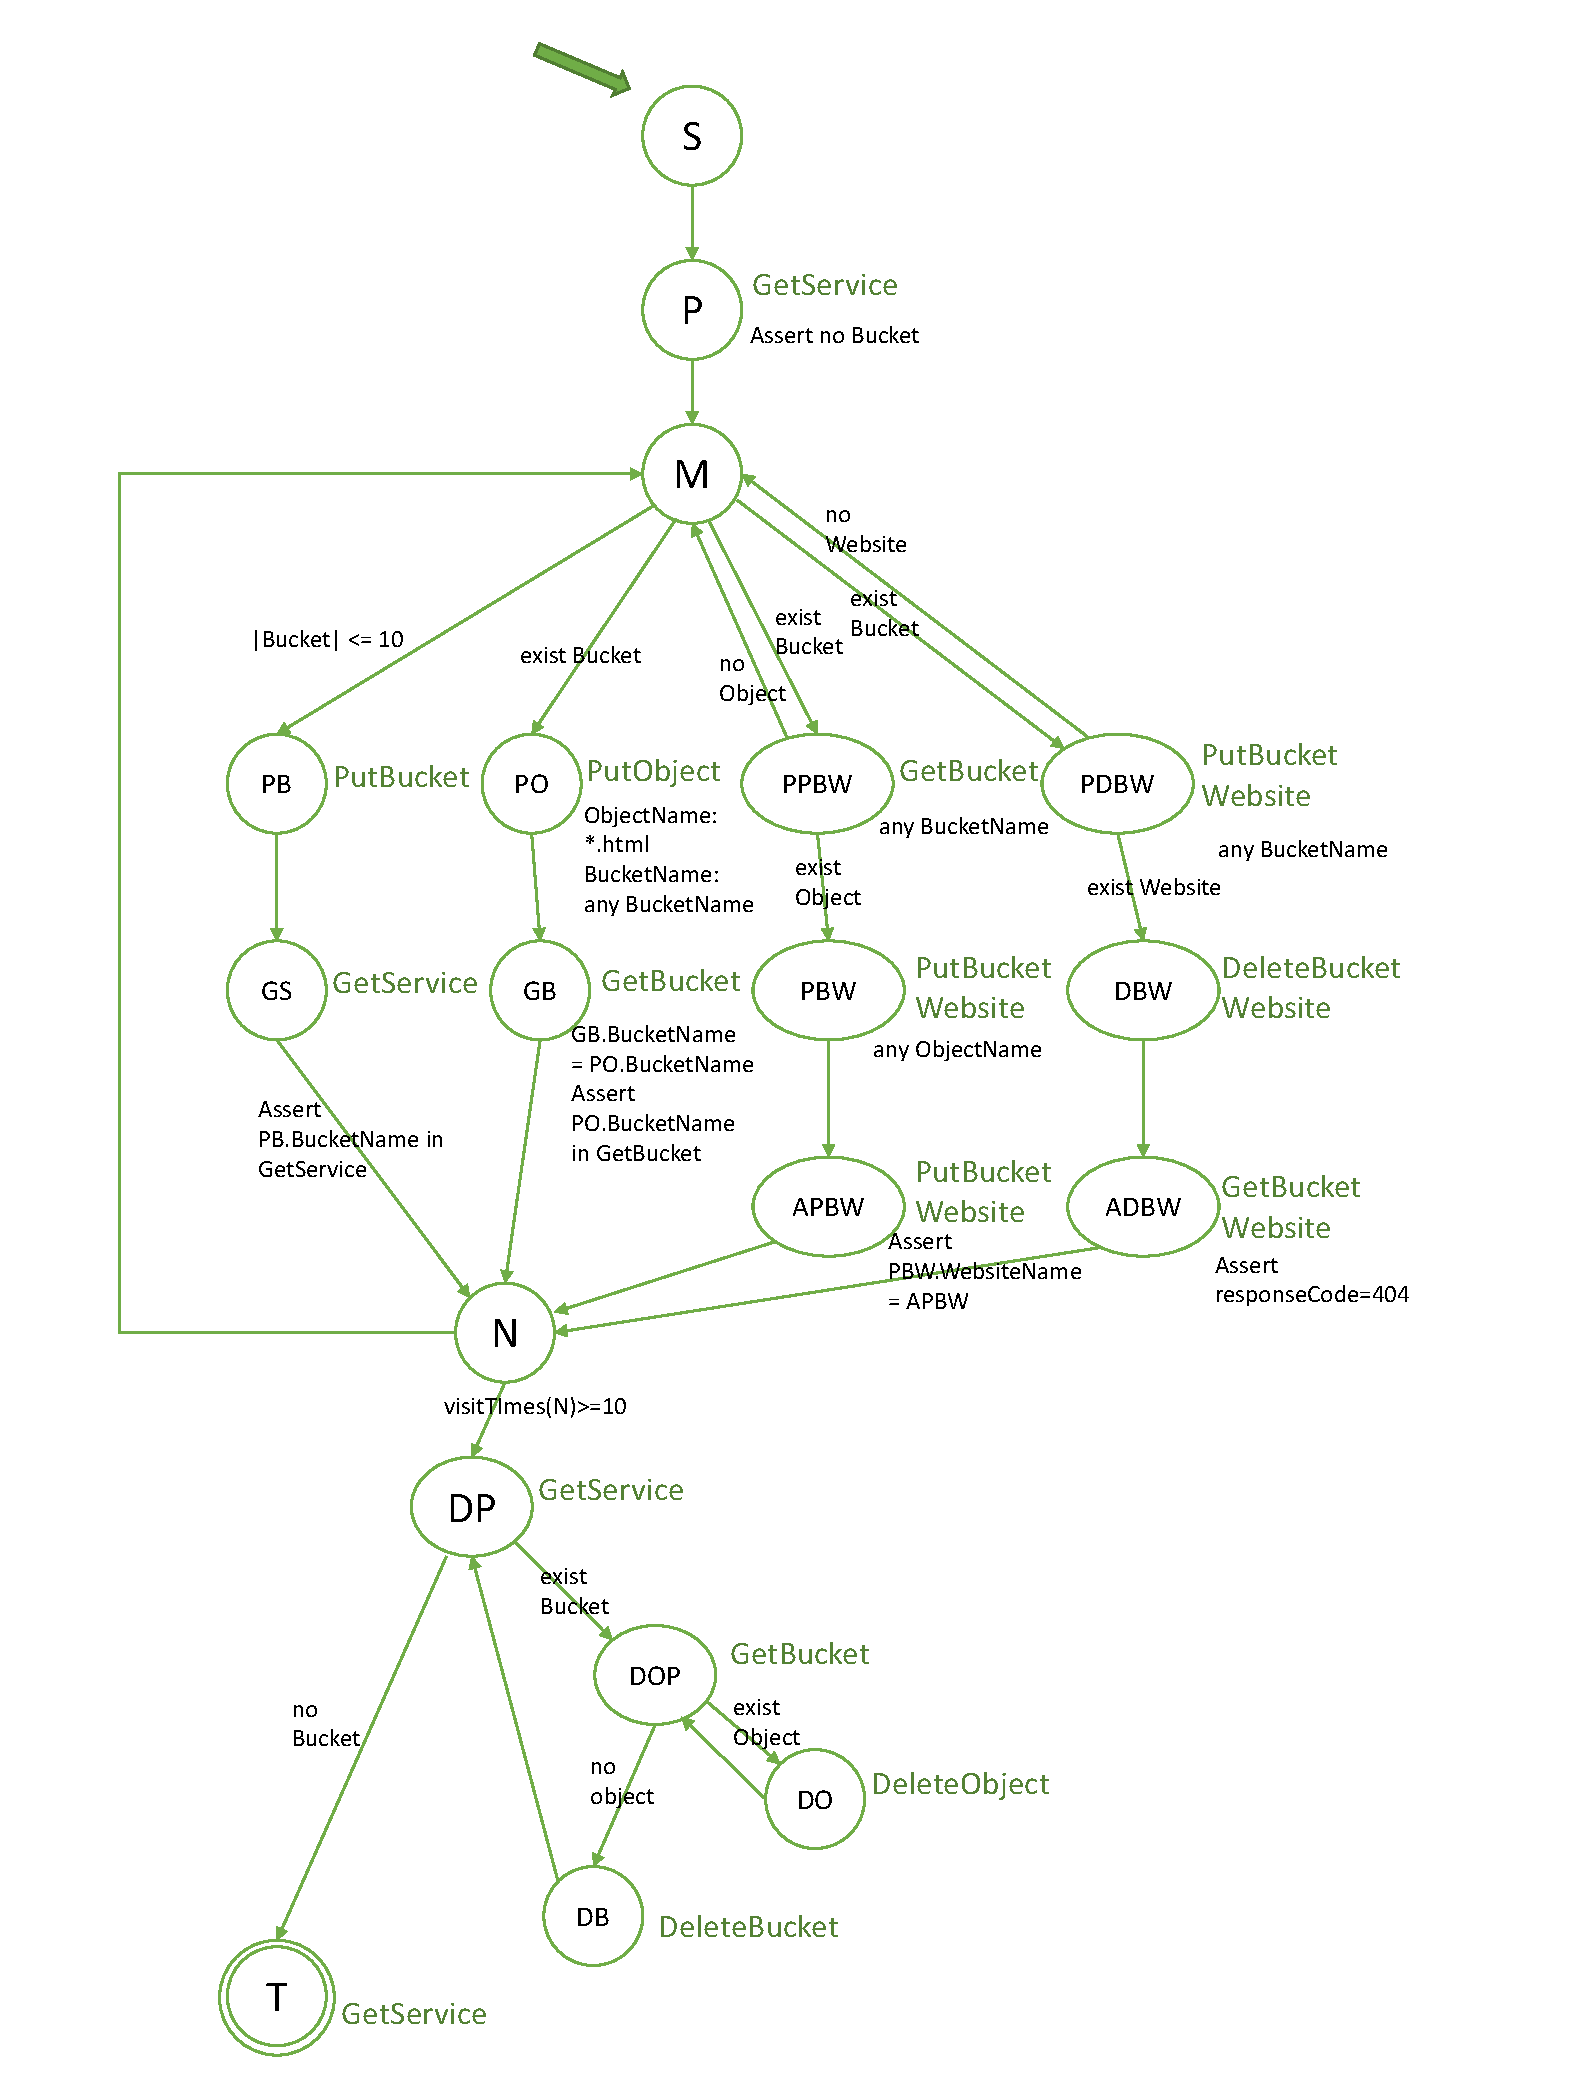
\includegraphics[width=400pt]{scenarioOSS_A.pdf}
            \caption{OSS(云对象存储服务) Scenario A.}
            \label{fig:oss_scenario_A}
        \end{figure}
        
         \begin{figure}[!htb]
            \centering
            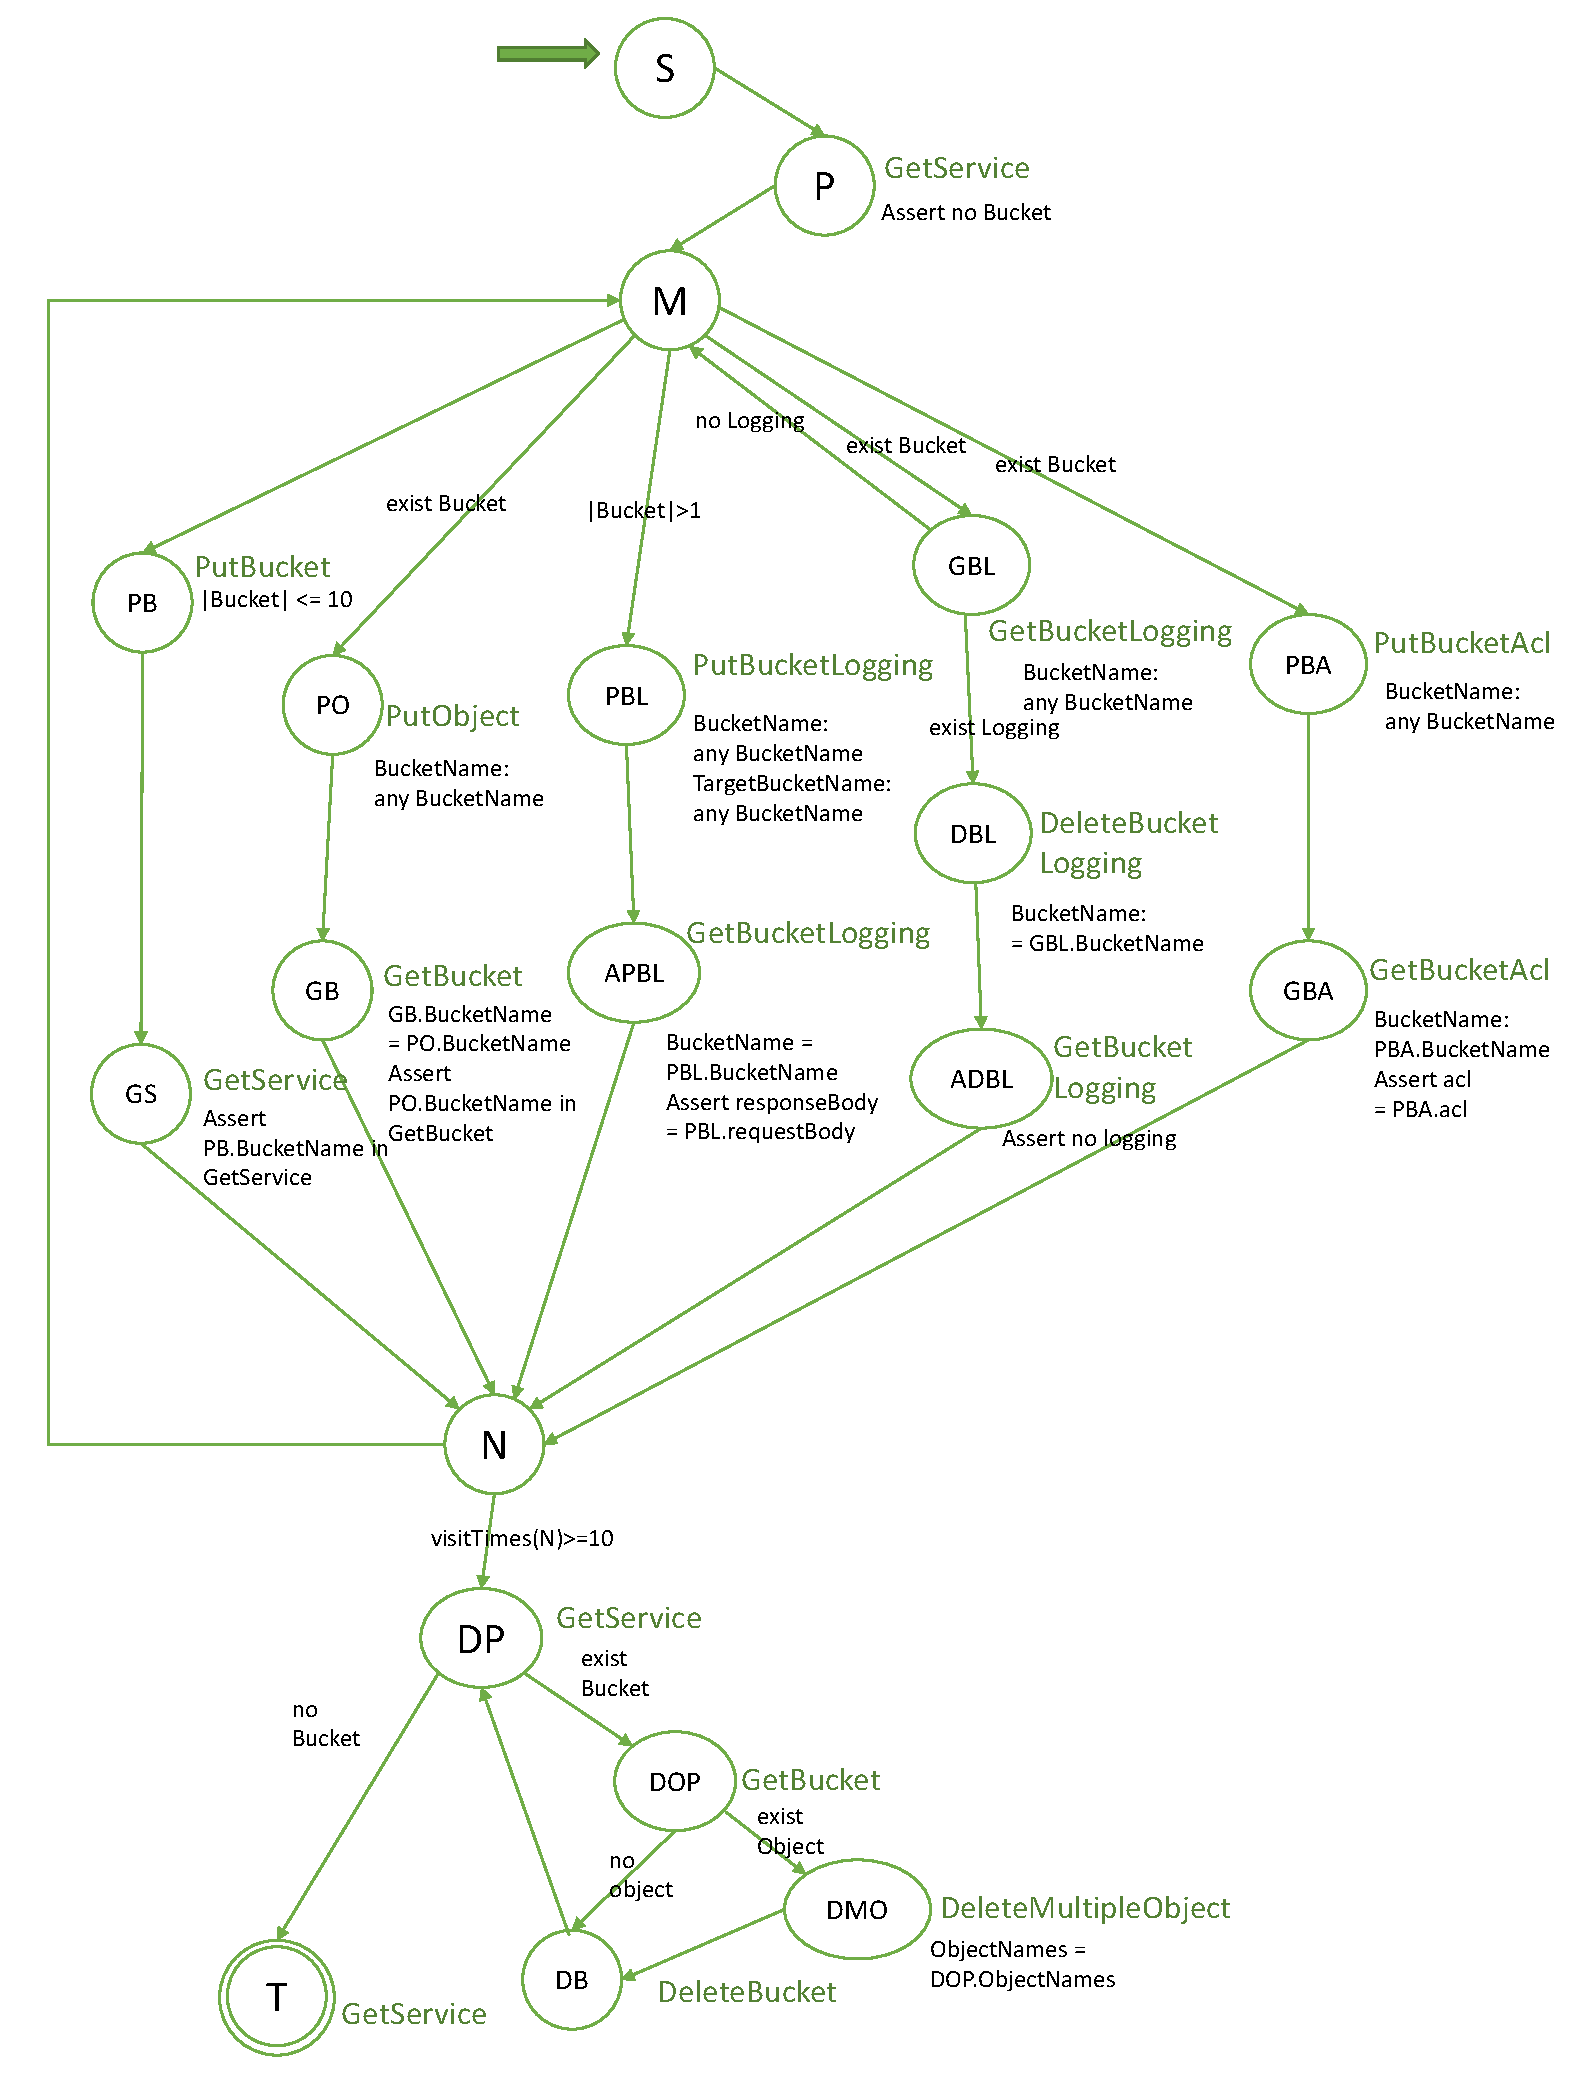
\includegraphics[width=400pt]{scenarioOSS_B.pdf}
            \caption{OSS(云对象存储服务) Scenario B.}
            \label{fig:oss_scenario_B}
        \end{figure}
        
         \begin{figure}[!htb]
            \centering
            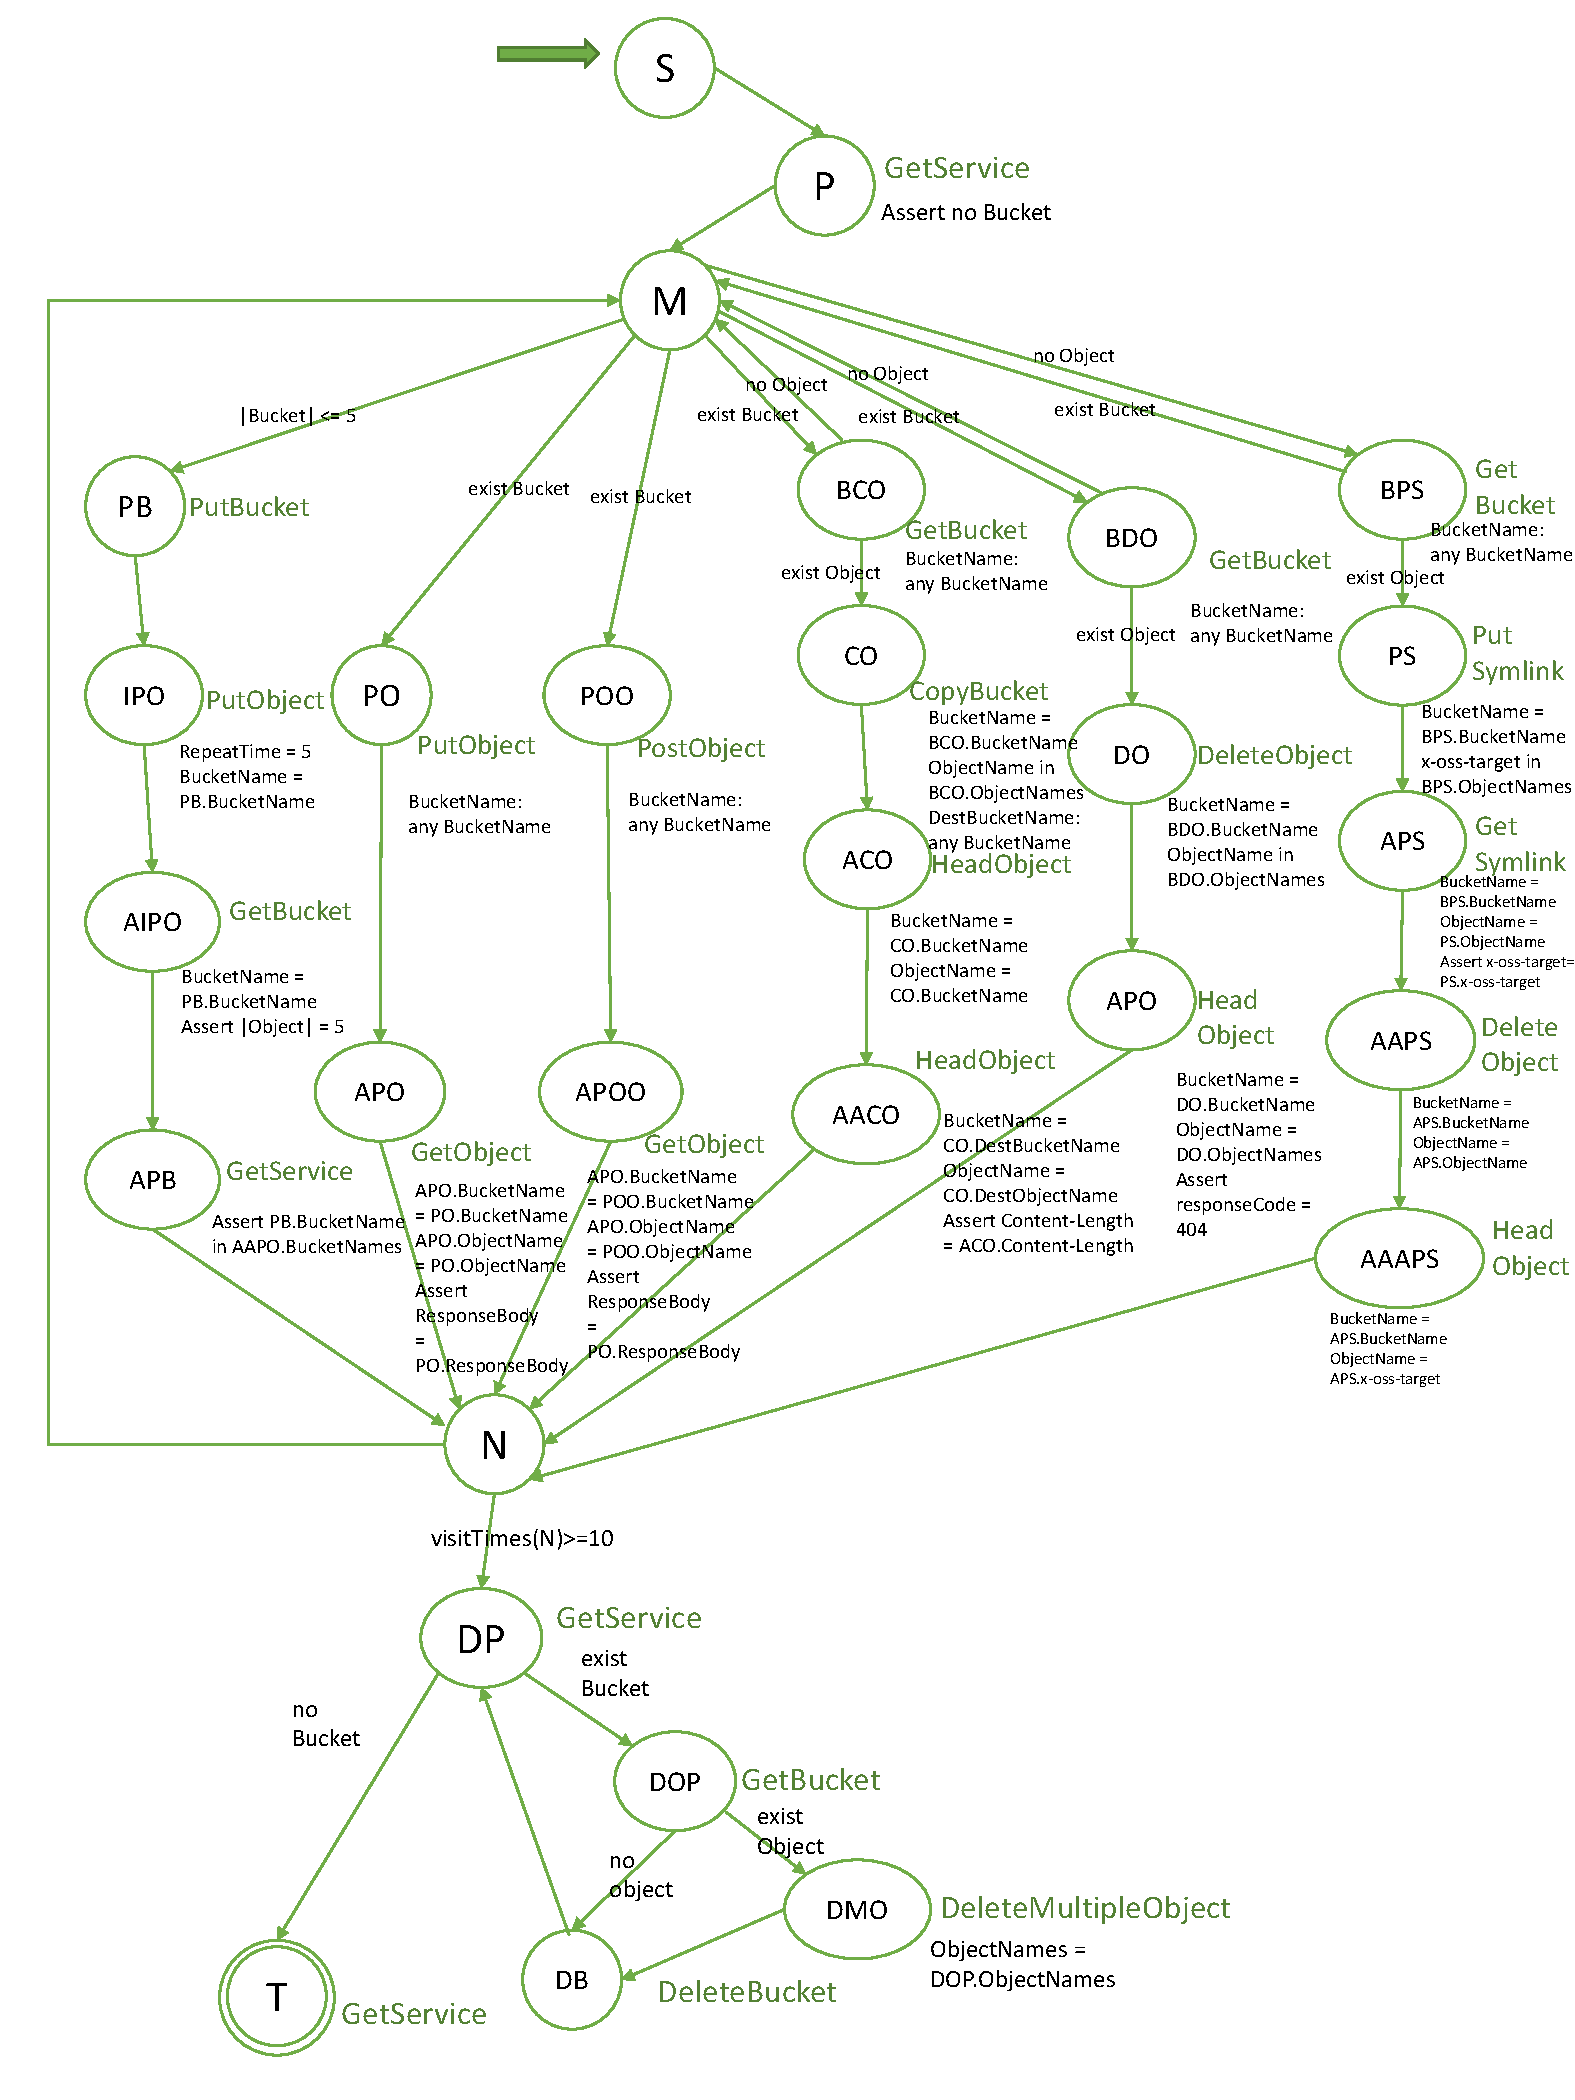
\includegraphics[width=400pt]{scenarioOSS_C.pdf}
            \caption{OSS(云对象存储服务) Scenario C.}
            \label{fig:oss_scenario_C}
        \end{figure}
    
    \section{ECS服务测试场景模型}
        ECS服务(云服务器服务)的场景模型仅一个, 见图\ref{fig:ecs_scenario}.
        
        \begin{figure}[!htb]
            \centering
            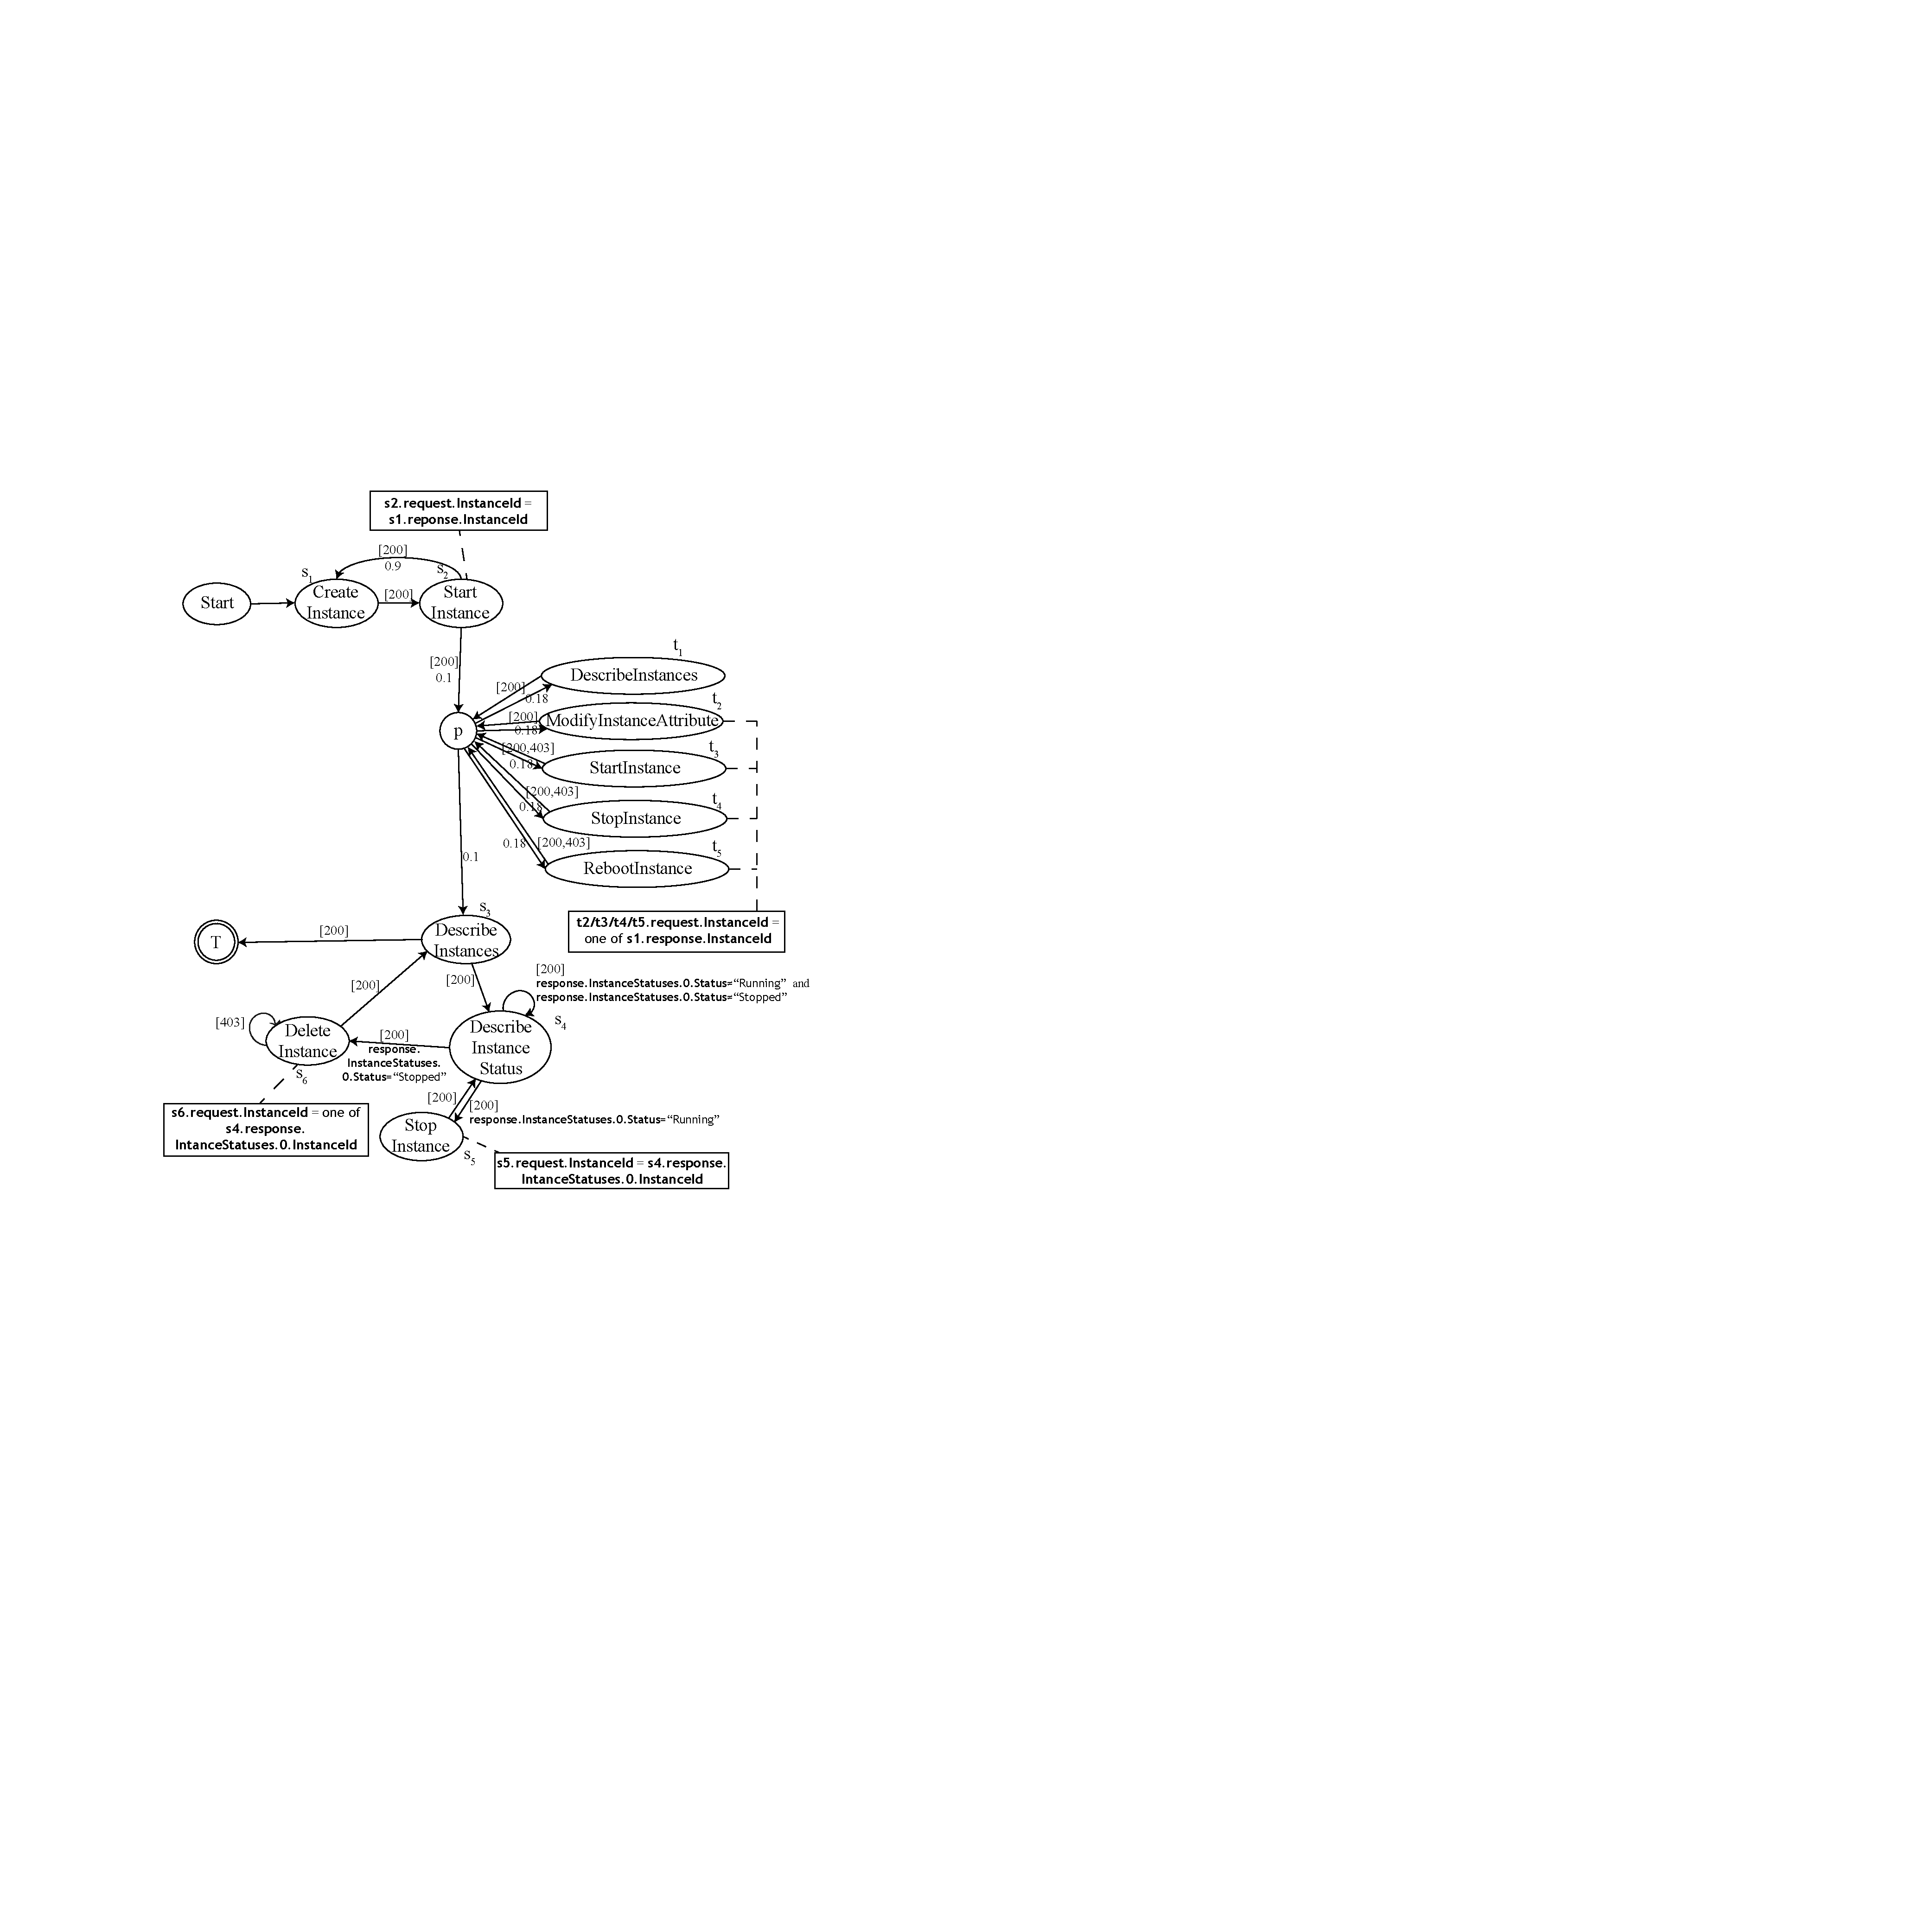
\includegraphics[width=400pt]{scenarioECS.pdf}
            \caption{ECS(云服务器服务)的场景模型.}
            \label{fig:ecs_scenario}
        \end{figure}
        
    \section{E-payment服务测试场景模型}
        \label{sec:epayment_scenario_model}
    
        E-payment服务(电子支付服务实时贷记API)的测试场景为链式, 该链式场景专用于分区测试数据的合成. 除了最后一个状态的其余状态均依次进行各个参数的生成, 为了引入数据分区, 各个参数的生成使用自定义生成函数, 自定义生成函数依照各个参数的数据分区随机生成参数. 最后一个状态对之前各个状态生成的参数进行合成, 即把各个参数合成为一个对象类型, 其各成员为之前生成的各参数, 此处引入数据依赖, 以从上下文中获取之前生成的参数. 最后一个状态与被测API关联, 发送合成对象作为请求数据. 示意图见\ref{fig:epayment_scenario}.
        
        \begin{figure}[!htb]
            \centering
            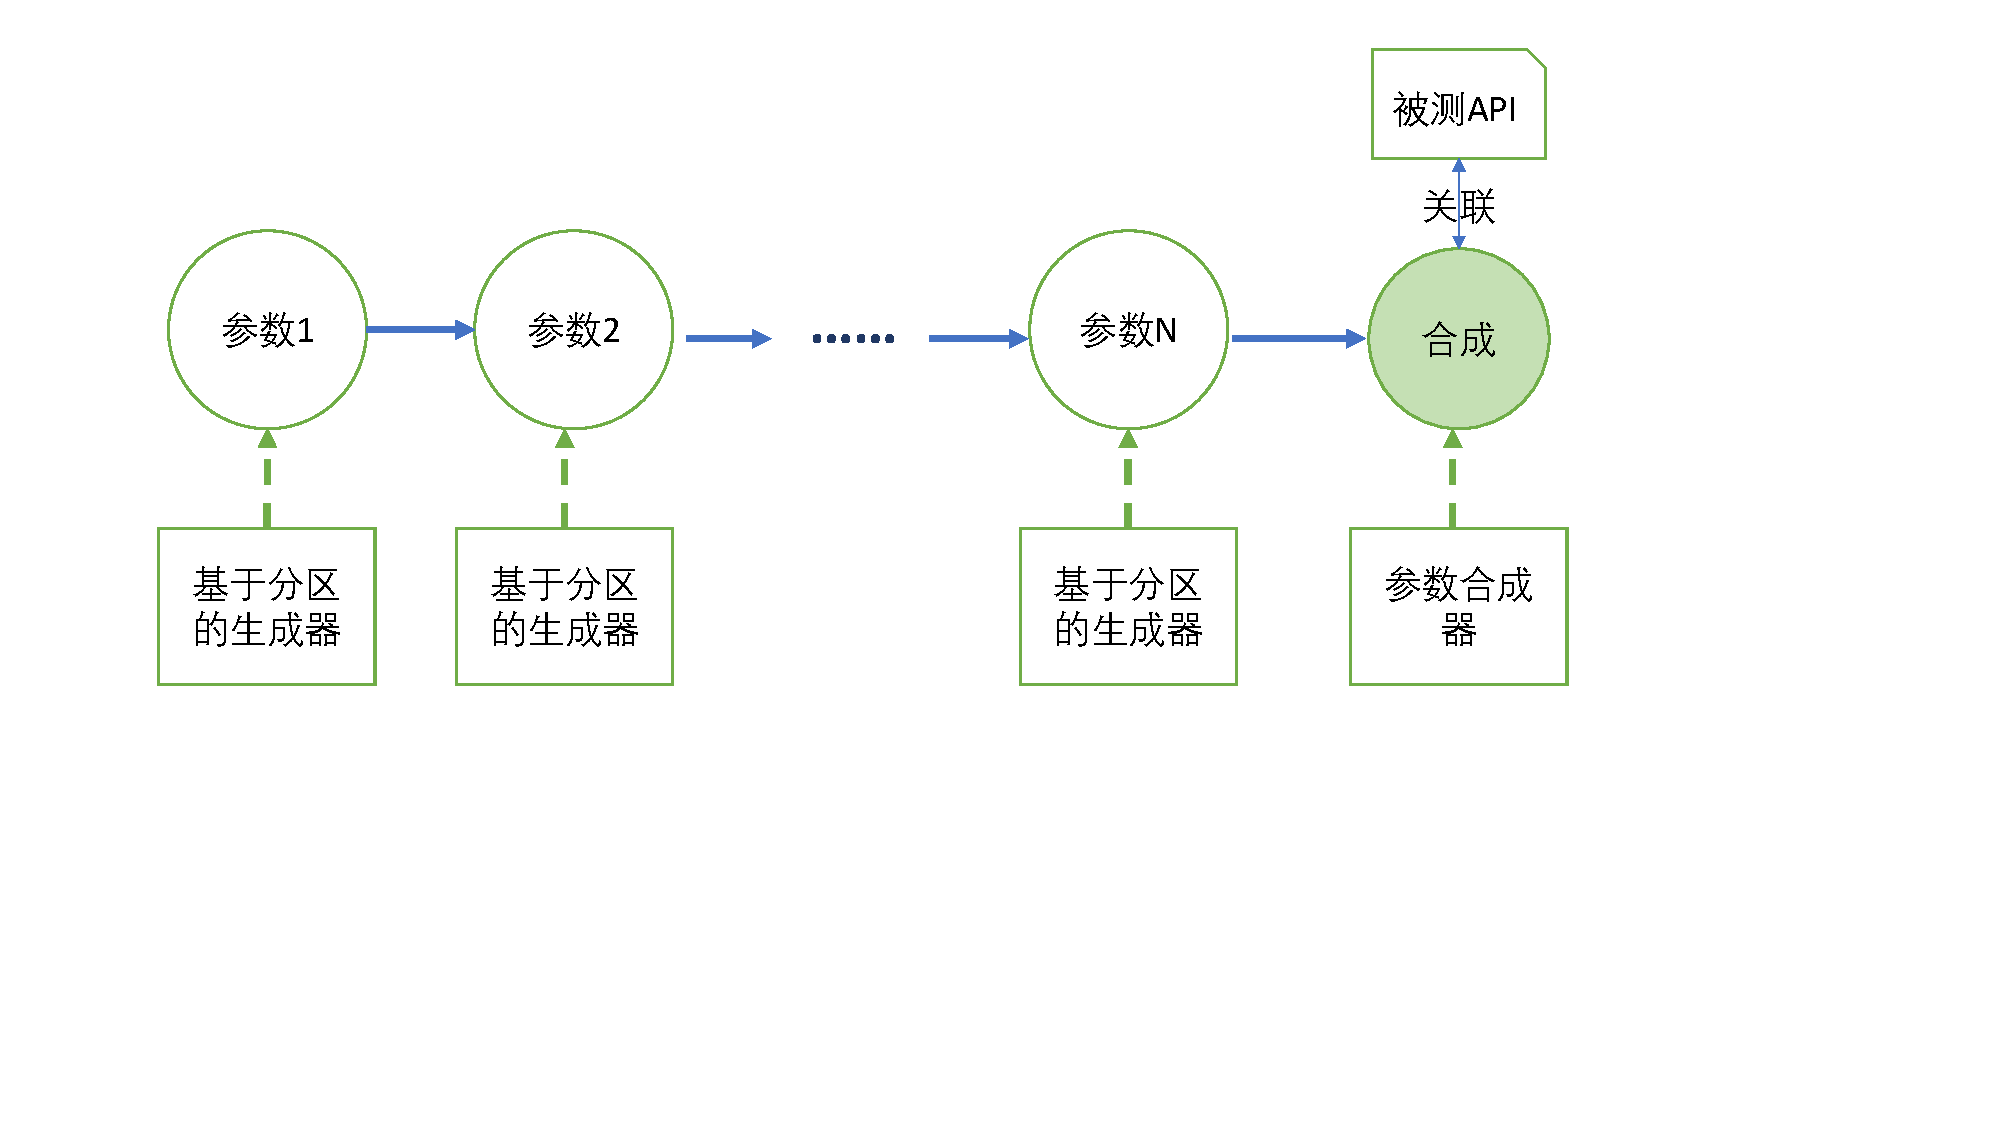
\includegraphics[width=400pt]{scenario_E-payment_pattern.pdf}
            \caption{E-payment的场景模型示意图. 该场景被设计为链式, 专用于分区测试数据的合成.}
            \label{fig:epayment_scenario}
        \end{figure}
        